\documentclass{article}
\usepackage{fancyhdr}
\usepackage{ctex}
\usepackage{listings}
\usepackage{graphicx}
\usepackage[a4paper, body={18cm,22cm}]{geometry}
\usepackage{amsmath,amssymb,amstext,wasysym,enumerate,graphicx}
\usepackage{float,abstract,booktabs,indentfirst,amsmath}
\usepackage{array}
\usepackage{booktabs}
\usepackage{multirow}
\usepackage{url}
\usepackage{diagbox}
\renewcommand\arraystretch{1.4}
\usepackage{indentfirst}
\setlength{\parindent}{2em}
\usepackage{enumitem}
\setmonofont{Consolas}
\usepackage{listings}
\usepackage{xcolor}
\usepackage{makecell}
\usepackage{tikz}
\usetikzlibrary{positioning, arrows.meta}
\setCJKmonofont{黑体}
\lstset{  
	% 基本设置  
	xleftmargin = 3em, xrightmargin = 3em, aboveskip = 1em,  
	backgroundcolor = \color{white},  
	basicstyle = \small\ttfamily,  
	rulesepcolor = \color{gray},  
	breaklines = true,  
	numbers = left,  
	numberstyle = \small,  
	numbersep = -14pt,  
	frame = shadowbox,  
	showspaces = false,  
	columns = fixed,  
	sensitive = true,  
	% VSCode 风格配色  
	keywordstyle = \color{blue!70!black}\bfseries,  
	emphstyle = \color{red!70!black}\bfseries, % 对于强调的词  
	emphstyle=[2]\color{purple!70!black}\bfseries, % 对于第二组强调的词  
	commentstyle = \color{green!60!black}, % 注释颜色  
	stringstyle = \color{orange!90!black}, % 字符串颜色更亮一些  
	morekeywords={ASSERT, int64\_t, uint32\_t},  
	moreemph={ASSERT, NULL},  
	moreemph=[2]{int64\_t, uint32\_t, tid\_t, uint8\_t, int16\_t, uint16\_t, int32\_t, size\_t, bool},  
	morecomment=[l][\color{green!60!black}]{+}, % 以+开头的注释  
}

%--------------------页眉--------------------%
\pagestyle{fancy}
\fancyhead[L]{}
\fancyhead[R]{}
\fancyhead[C]{答题模板}
\fancyfoot[C]{-\thepage-}
\renewcommand{\headrulewidth}{1.5pt}
%--------------------标题--------------------%
\begin{document}
\begin{center}
	{\Large{\textbf{\heiti 软件质量分析期末考试}}}
	\begin{table}[H]
		\centering
		\begin{tabular}{p{2cm}p{4cm}<{\centering}p{1cm}p{2cm}p{6cm}<{\centering}}
			课程名称:    & 软件质量分析 & \quad & 指导教师:    & 陈仪香
			\\ \cline{2-2} \cline{5-5}
			姓\qquad 名: & 王海生    & \quad & 学\qquad 号: & 10235101559
			\\ \cline{2-2} \cline{5-5}
			年\qquad 级: & 2023级    & \quad & 主\qquad 题: & 期末考试
			\\ \cline{2-2} \cline{5-5}
		\end{tabular}
	\end{table}
	
	% 添加新行并居中
	%\vspace{1em} % 可选:添加垂直间距
\end{center}
\rule{\textwidth}{1pt}

\tableofcontents

%--------------------正文--------------------%
\section{hw5-软件可信度量模型-模型1}

\subsection{题目}

设软件$ S $有五个属性,譬如功能性(Functionality)、安全性(Safety)、可靠性(Reliability)、生存性(Survivability)、可维护性(Maintainability),分别使用字母$ F $、$ SF $、$ R $、$ SV $、$ M $表示。使用上述软件可信度量模型,利用给定数据,计算最后一列$ T $。

权重系数表:

\begin{center}
	\begin{tabular}{|c|c|c|c|c|}
		\hline
		$ \alpha_F $ & $ \alpha_{SF} $ & $ \alpha_R $ & $ \alpha_{SV} $ & $ \alpha_M $ \\ \hline
		0.25          & 0.15             & 0.20           & 0.23             & 0.17           \\ \hline
	\end{tabular}
\end{center}

属性评分表:

\begin{center}
	\begin{tabular}{|c|c|c|c|c|c|}
		\hline
		$ F $ & $ SF $ & $ R $ & $ SV $ & $ M $ & $ T $ \\ \hline
		6.8     & 8.2      & 7.8     & 6.8      & 7.9     &         \\ \hline
		8.8     & 8.9      & 9.2     & 9.0      & 9.3     &         \\ \hline
		5.6     & 5.9      & 6.0     & 9.0      & 5.3     &         \\ \hline
		4.6     & 7.8      & 3.8     & 5.1      & 4.5     &         \\ \hline
	\end{tabular}
\end{center}

\subsection{相关知识点}

可信度量模型-模型1表述如下:

$$
T_1 = \frac{10}{11}\left(\frac{y_{\text{min}}}{10}\right)^\epsilon y^{\alpha_1}_1 y^{\alpha_2}_2 \cdots y^{\alpha_m}_m + \frac{10}{11} y^{\beta_{m+1}}_{m+1} y^{\beta_{m+2}}_{m+2} \cdots y^{\beta_{m+s}}_{m+s}
$$

其中:
\begin{itemize}
	\item $0 \leq \epsilon \leq 1 - \alpha_{\text{min}}$ 控制最小关键属性对软件可信度的影响。
	\item $1 \leq y_i \leq 10, 1 \leq i \leq m+s$ 是每个属性的值范围。
	\item $y_{\text{min}} = \min\{y_i | i=1, \cdots, m\}$ 是所有关键属性中的最小值。
\end{itemize}

\subsection{\texttt{Python}代码}

\begin{lstlisting}[language=Python]
	# 插入代码
\end{lstlisting}

\subsection{答案}

\subsubsection{代码运行结果}

\begin{figure}[H]
	\centering
	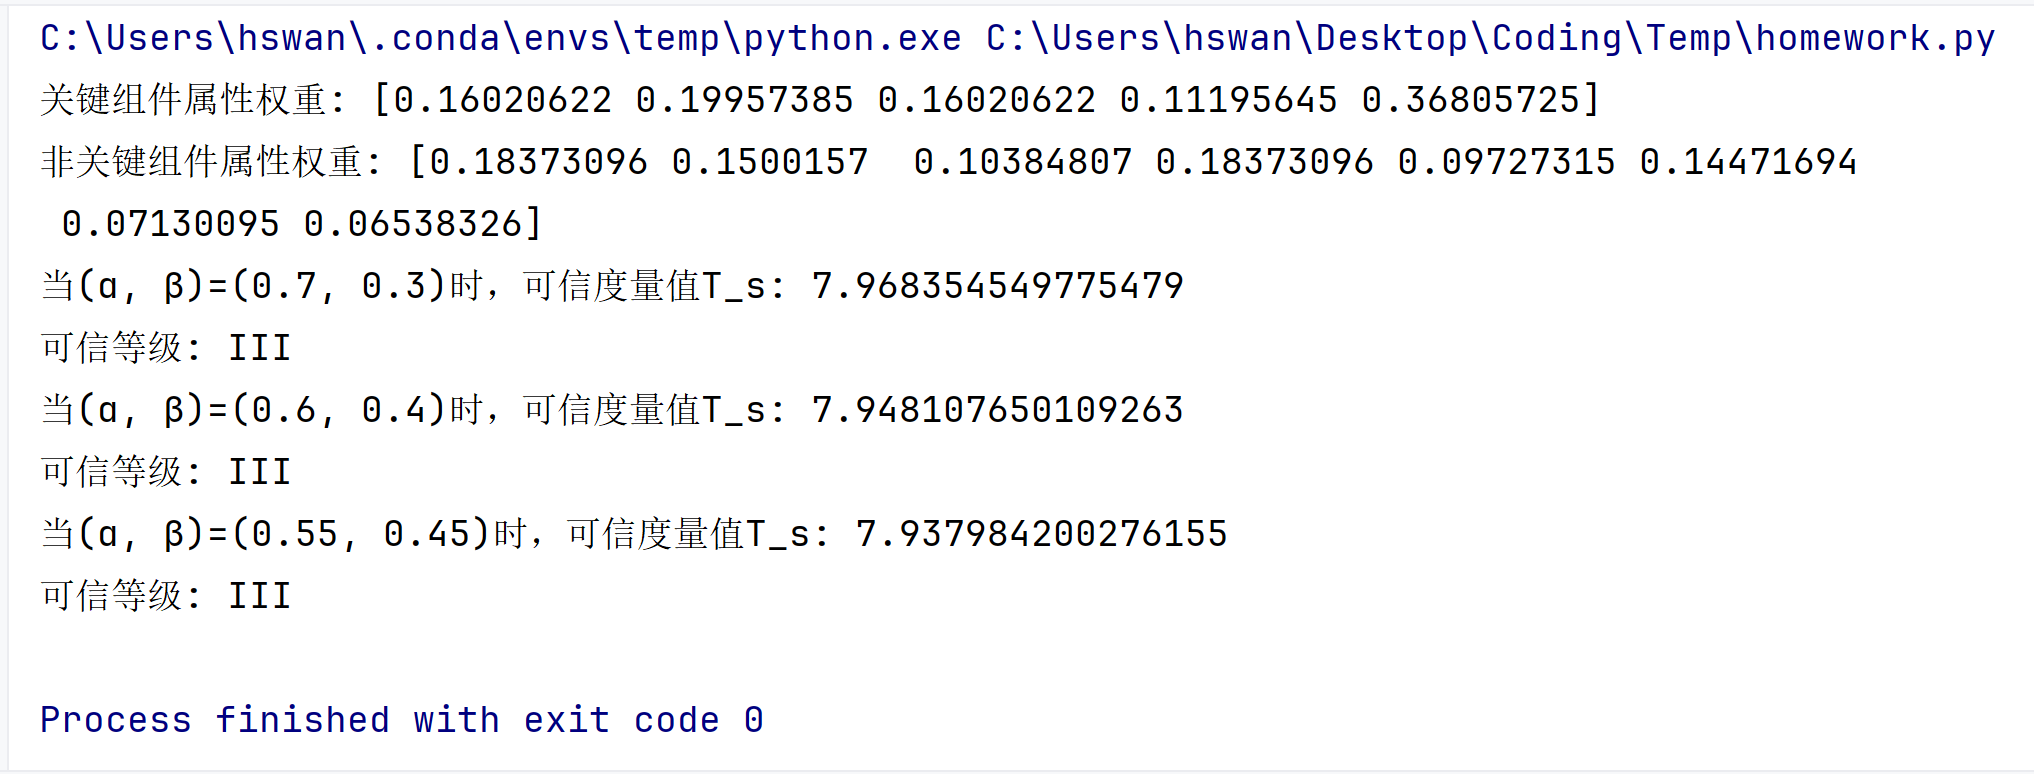
\includegraphics[width=0.9\textwidth]{img/1.png}
	\caption{运行结果}
\end{figure}

\subsubsection{题目答案}

\begin{center}
	\begin{tabular}{|c|c|c|c|c|c|}
		\hline
		$ F $ & $ SF $ & $ R $ & $ SV $ & $ M $ & $ T $ \\ \hline
		6.8     & 8.2      & 7.8     & 6.8      & 7.9     & 7.3738        \\ \hline
		8.8     & 8.9      & 9.2     & 9.0      & 9.3     & 9.0241        \\ \hline
		5.6     & 5.9      & 6.0     & 9.0      & 5.3     & 6.3228        \\ \hline
		4.6     & 7.8      & 3.8     & 5.1      & 4.5     & 4.8893        \\ \hline
	\end{tabular}
\end{center}









\section{hw5-软件可信度量模型-模型3}

\subsection{题目}

设有4个软件系统,分别编号为1、2、3、4。它们都有7个属性,其中4个为关键属性,编号为$y_1,y_2,y_3,y_4$,其权重分别为$\alpha_1 = 0.3$,$\alpha_2 = 0.2$,$\alpha_3 = 0.35$,$\alpha_4 = 0.15$。3个为非关键属性,编号为$y_5,y_6,y_7$,其权重分别为$\beta_1 = 0.35$,$\beta_2 = 0.40$,$\beta_3 = 0.25$。关键属性权重$\alpha = 0.70$,非关键属性$\beta = 0.30$。依据下表的各属性取值,使用模型$T_3$计算各软件的可信性度值。

\begin{center}
	\begin{tabular}{|c|c|c|c|c|c|c|c|c|c|c|}
		\hline
		编号 & $y_1$ & $y_2$ & $y_3$ & $y_4$ & $y_5$ & $y_6$ & $y_7$ & $\varepsilon$ & $\rho$ & $T_3$ \\ \hline
		1   & 8.3   & 7.1   & 8.1   & 6.9   & 9.1   & 8.5   & 8.6   & 0.1           & 0.10   &       \\ \hline
		2   & 7.8   & 8.7   & 8.0   & 6.2   & 8.9   & 8     & 8.8   & 0.05          & 0.15   &       \\ \hline
		3   & 5.8   & 8.1   & 6.8   & 5.6   & 7.9   & 6.8   & 8.1   & 0.1           & 0.10   &       \\ \hline
		4   & 6.8   & 7.8   & 8.1   & 6.9   & 8.9   & 7.8   & 8.8   & 0.05          & 0.15   &       \\ \hline
		5   & 3.8   & 3.7   & 4.8   & 4.7   & 3.9   & 5.8   & 6.8   & 0.1           & 0.10   &       \\ \hline
		6   & 8.4   & 7.2   & 8.1   & 7.7   & 7.9   & 8.8   & 6.8   & 0.05          & 0.15   &       \\ \hline
		7   & 9.0   & 8.7   & 8.9   & 8.6   & 9.1   & 8.8   & 8.9   & 0.1           & 0.10   &       \\ \hline
		8   & 8.0   & 7.8   & 6.8   & 8.7   & 7.9   & 8.1   & 8.3   & 0.05          & 0.15   &       \\ \hline
	\end{tabular}
\end{center}

\subsection{相关知识点}

可信度量模型-模型3表述如下:

$$
T_3 = \left\{ \alpha \left[ \min_{1 \leq i \leq m} \left( \frac{y_i}{10} \right)^\epsilon y_1^{\alpha_1} y_2^{\alpha_2} \cdots y_m^{\alpha_m} \right]^{-\rho} + \beta \left[ y_{m+1}^{\beta_{m+1}} y_{m+2}^{\beta_{m+2}} \cdots y_{m+s}^{\beta_{m+s}} \right]^{-\rho} \right\}^{-\frac{1}{\rho}}
$$

其中,

\begin{itemize}
	\item $\epsilon$:调控参数,用来调控最小关键属性对软件可信性的影响,满足 $0 \leq \epsilon \leq \min\{1 - \alpha_{\text{min}}', \frac{\ln y_0 - \ln y_{\text{min}}'}{\ln y_{\text{min}}' - \ln 10}\}$,且$\epsilon$越大,影响越大。这里,$\alpha_{\text{min}}'$ 表示最小关键属性在整个关键属性集中所占的权重;
	\item $y_0$:由用户提供的可信属性值需达到的阈值;
	\item $\rho$:与关键属性和非关键属性之间替代性相关的参数,满足 $0 < \rho$,其值越大,则关键属性与非关键属性间替代性越难;
	\item $y_i$:第$i(1 \leq i \leq m + s)$个可信属性的可信值,满足 $1 \leq y_0 \leq y_i \leq 10$。
\end{itemize}

\subsection{\texttt{Python}代码}

\begin{lstlisting}[language=Python]
	# 插入代码
\end{lstlisting}

\subsection{答案}

\subsubsection{代码运行结果}

\begin{figure}[H]
	\centering
	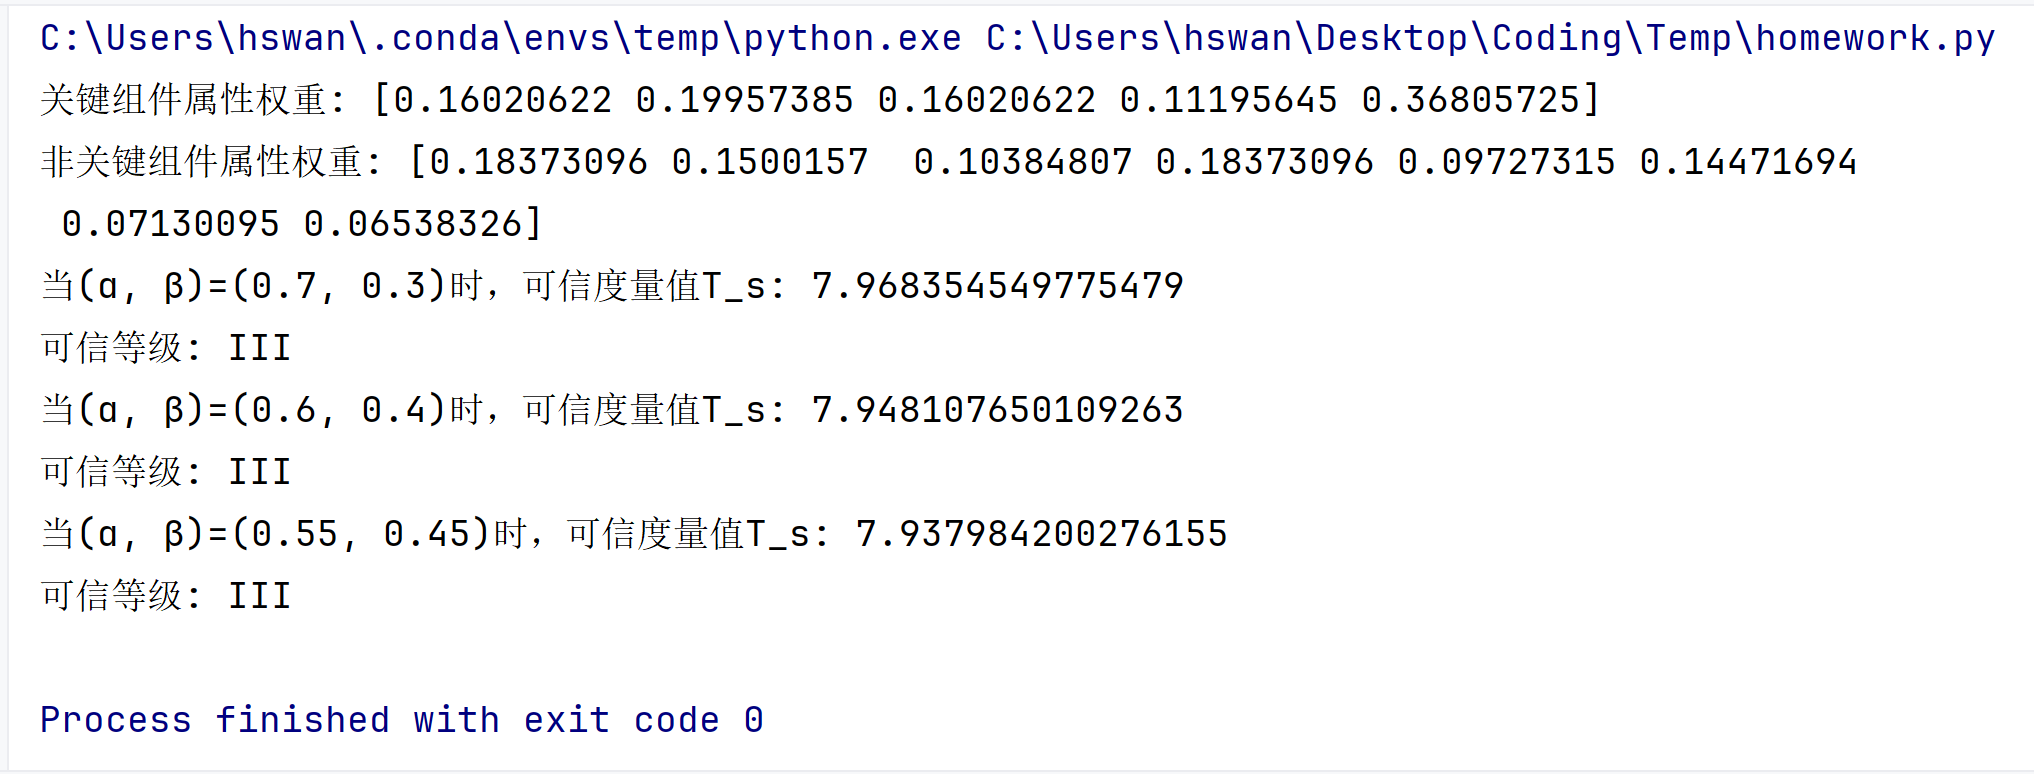
\includegraphics[width=0.9\textwidth]{img/1.png}
	\caption{运行结果}
\end{figure}

\subsubsection{题目答案}













\section{hw6-软件可信属性度量模型}

\subsection{题目}

设有4个软件系统,分别编号为1,2,3,4。它们都有可靠性属性$y$,含有5个子属性,编号为$x_1, x_2, x_3, x_4, x_5$,其权重分别为$\gamma_1(\omega_1) = 0.15$, $\gamma_2(\omega_2) = 0.20$, $\gamma_3(\omega_3) = 0.20$, $\gamma_4(\omega_4) = 0.25$, $\gamma_5(\omega_5) = 0.20$。参数$\rho_y = \{0.01, 0.55\}$。按照模型1($y_1$)和模型2($y_2$)分别计算可靠性属性$y$的可信度量值,注意:模型1是不需要参数$\rho_y$的。

\begin{center}
	\begin{tabular}{|c|c|c|c|c|c|c|c|c|}
		\hline
		编号 & $x_1$ & $x_2$ & $x_3$ & $x_4$ & $x_5$ & $\rho_y$ & $y_1$ & $y_2$ \\ \hline
		1   & 8.6   & 9.1   & 9.2   & 8.8   & 8.9   & 0.01     &       &       \\ \cline{2-9}
		& 8.6   & 9.1   & 9.2   & 8.8   & 9.9   & 0.55     &       &       \\ \hline
		2   & 6.8   & 7.9   & 5.9   & 6.6   & 6.1   & 0.01     &       &       \\ \cline{2-9}
		& 6.8   & 7.9   & 5.9   & 6.6   & 6.1   & 0.55     &       &       \\ \hline
		3   & 9.1   & 9.9   & 8.9   & 8.8   & 7.8   & 0.01     &       &       \\ \cline{2-9}
		& 9.1   & 9.9   & 8.9   & 8.8   & 7.8   & 0.55     &       &       \\ \hline
		4   & 3.5   & 4.2   & 5.6   & 4.9   & 5.2   & 0.01     &       &       \\ \cline{2-9}
		& 3.5   & 4.2   & 5.6   & 4.9   & 5.2   & 0.55     &       &       \\ \hline
	\end{tabular}
\end{center}

\subsection{相关知识点}

\textbf{模型1}:

$$
y_1 = x_1^{\gamma_1} x_2^{\gamma_2} \cdots x_n^{\gamma_n}
$$

\textbf{模型2}:

$$
y_2 = \left( \sum_{i=1}^n \omega_i x_i^{-\rho_y} \right)^{-\frac{1}{\rho_y}}, \quad 1 \leq i \leq n, \quad 1 \leq x_i \leq 10
$$

其中,
\begin{itemize}
	\item $\rho_y$:与可信属性$y$相匹配的参数,它是构成可信属性$y$的可信子属性间替代性相关的参数,满足$\rho_y > 0$,且其值越大,则可信子属性间替代性越难。
	\item $\omega_i$:可信属性$y$的可信子属性$x_i \, (1 \leq i \leq n)$权重,满足 
	$$
	\sum_{i=1}^n \omega_i = 1, \quad 0 \leq \omega_i \leq 1.
	$$
\end{itemize}

\subsection{\texttt{Python}代码}

\begin{lstlisting}[language=Python]
	# 插入代码
\end{lstlisting}

\subsection{答案}

\subsubsection{代码运行结果}

\begin{figure}[H]
	\centering
	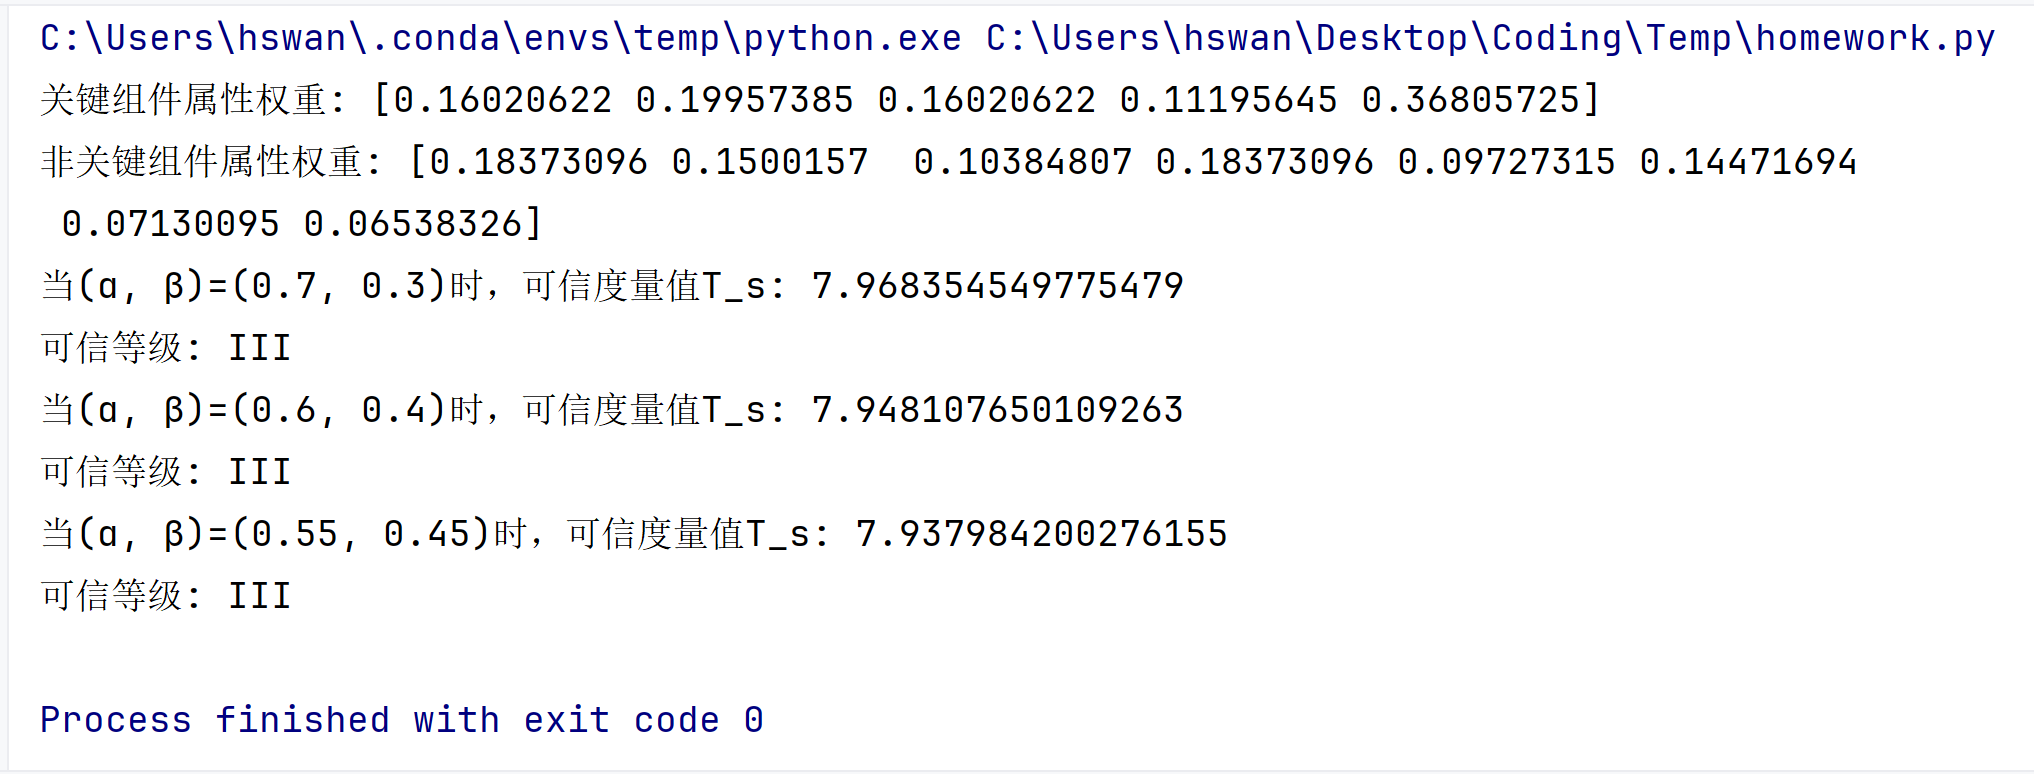
\includegraphics[width=0.9\textwidth]{img/1.png}
	\caption{运行结果}
\end{figure}

\subsubsection{题目答案}
















\section{hw6-权重向量}

\subsection{题目}

设\texttt{C919}飞行控制软件有5个可信属性:实时性、可靠性、可生存性、可维护性、功能性(其含义见第4讲第3.2节),其正互反判断矩阵$A$为

$$
A = \begin{bmatrix}
	1 & 1/2 & 3 & 2 & 1/2 \\
	2 & 1 & 2 & 3 & 2 \\
	1/3 & 1/2 & 1 & 2 & 1/3 \\
	1/2 & 1/3 & 1/2 & 1 & 2 \\
	2 & 1/2 & 3 & 1/2 & 1
\end{bmatrix}
$$

分别使用右特征向量法EV、对数最小二乘法LLSM、卡方最小二乘法CSM求出权重向量$W^{EV}$、$W^{LLSM}$、$W^{CSM}$,在此基础上使用“强度”方法求出最优的权重向量。

\subsection{相关知识点}

对于给定的正互反判断矩阵$A$,可以通过下面三种方法来估算权重向量:

\begin{enumerate}
	\item 右特征向量法(EigenVector Method, EV)
	\item 对数最小二乘法(Logarithmic Least Squares Method, LLSM)
	\item 卡方最小二乘法(Chi-Square Minimization Method, CSM)。
\end{enumerate}

最终应当选择\texttt{TD}值最小的方法。

\subsection{\texttt{Python}代码}

\begin{lstlisting}[language=Python]
	# 插入代码
\end{lstlisting}

\subsection{答案}

\subsubsection{代码运行结果}

\begin{figure}[H]
	\centering
	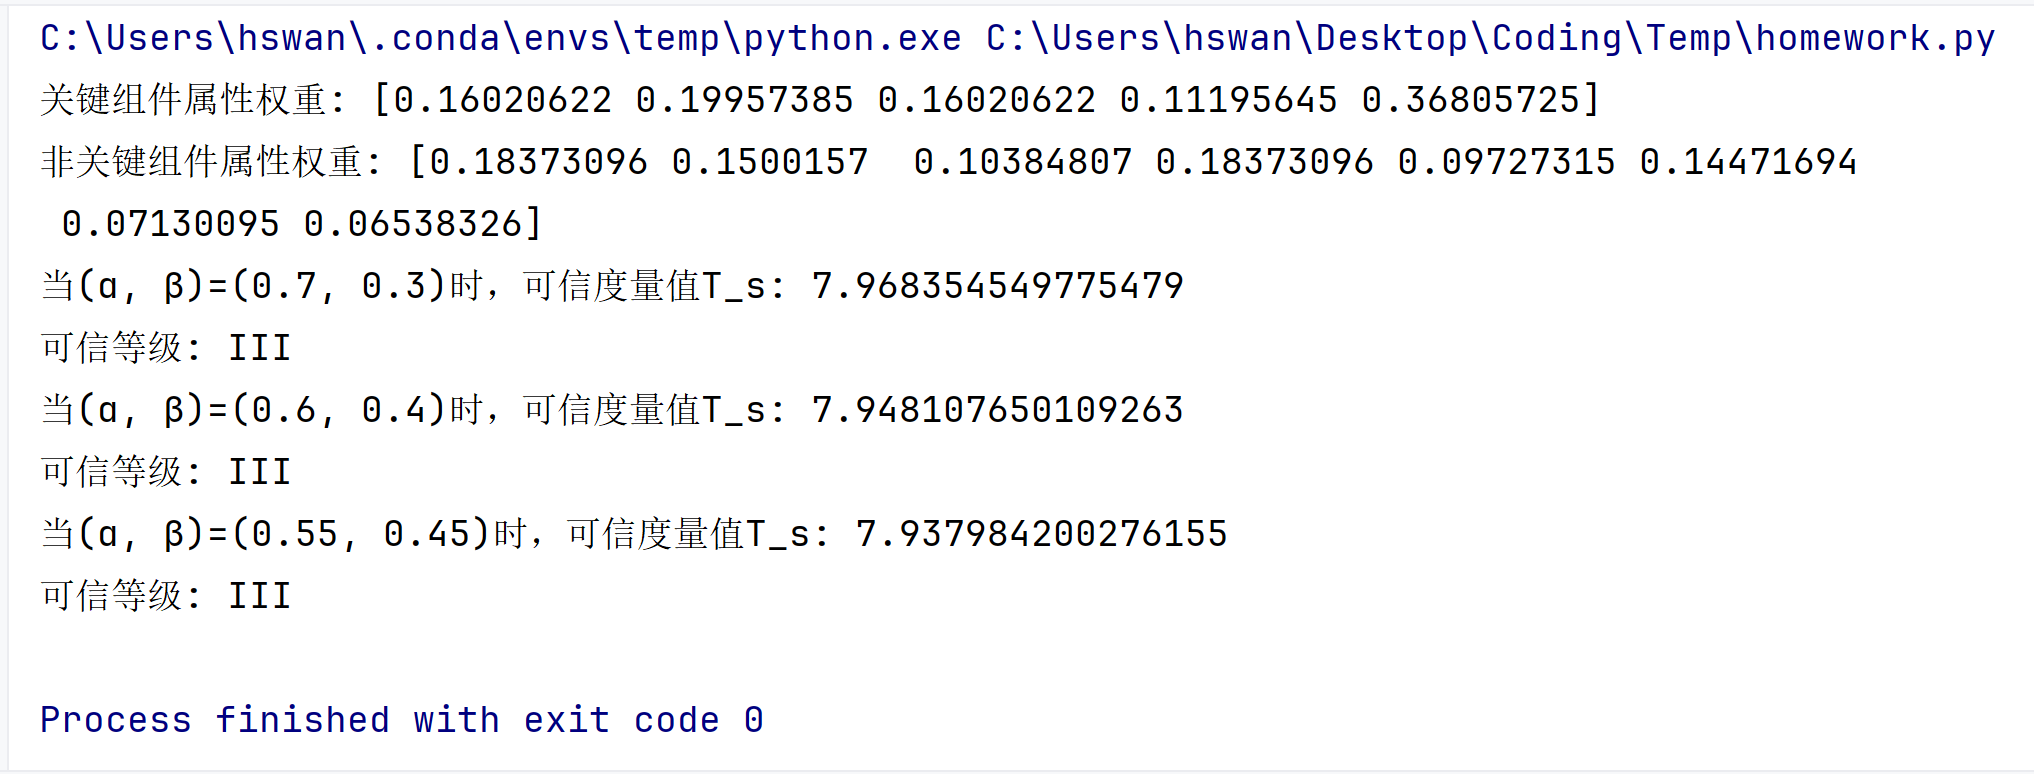
\includegraphics[width=0.9\textwidth]{img/1.png}
	\caption{运行结果}
\end{figure}

\subsubsection{题目答案}














\section{hw7-可信等级判定}

\subsection{题目}

依据下表中的数据,计算编号10-17软件的可信属性度量值、软件可信度量值以及可信等级。可信属性权重和子属性权重同例子一样。从可信属性度量值计算以及软件可信度量值计算模型都使用幂积公式。

——在这里直接插入题目图片——

\begin{figure}[H]
	\centering
	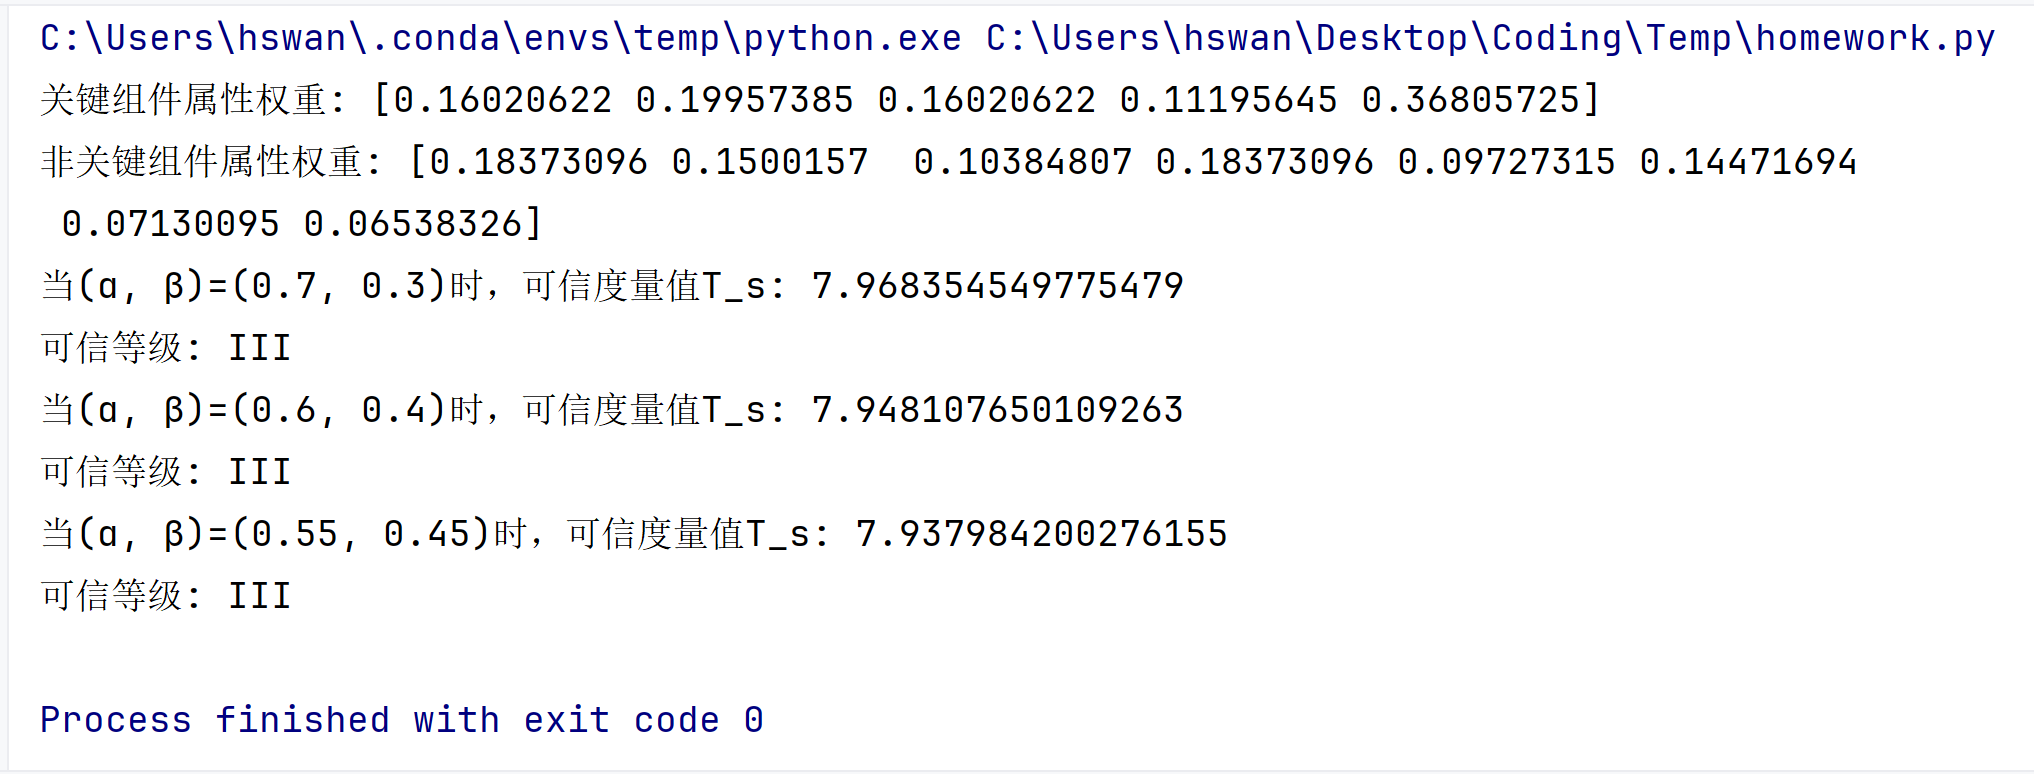
\includegraphics[width=0.9\textwidth]{img/1.png}
\end{figure}

\subsection{相关知识点}

\begin{figure}[H]
	\centering
	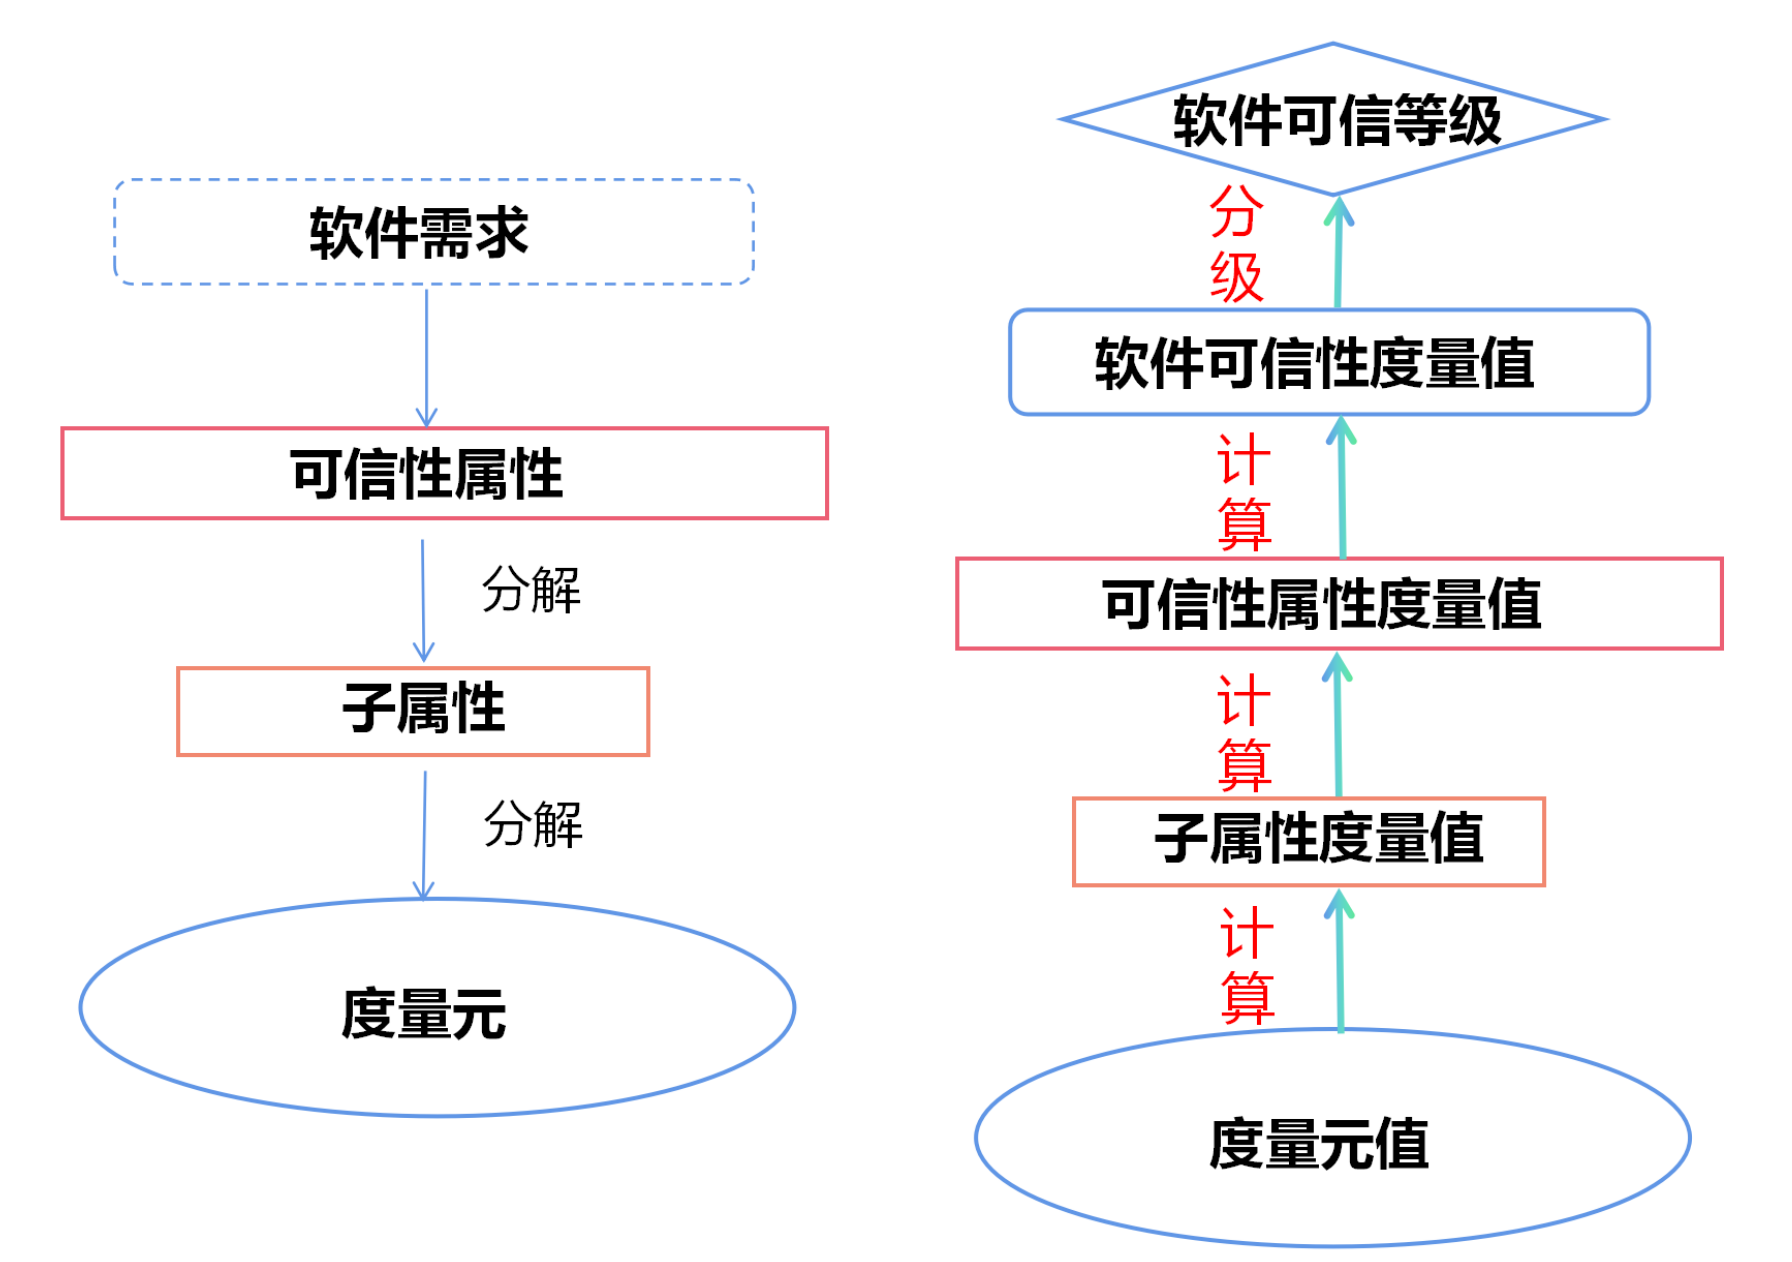
\includegraphics[width=0.6\textwidth]{img/static_1.png}
\end{figure}

由课堂内容可知,分析一个软件的可信等级,需要先自上而下地将软件需求解构为可信性属性、子属性、度量元;在计算时,要自下而上地计算每一个子类,然后得到最终的可信等级。更细节的流程图如下所示。

\begin{figure}[H]
	\centering
	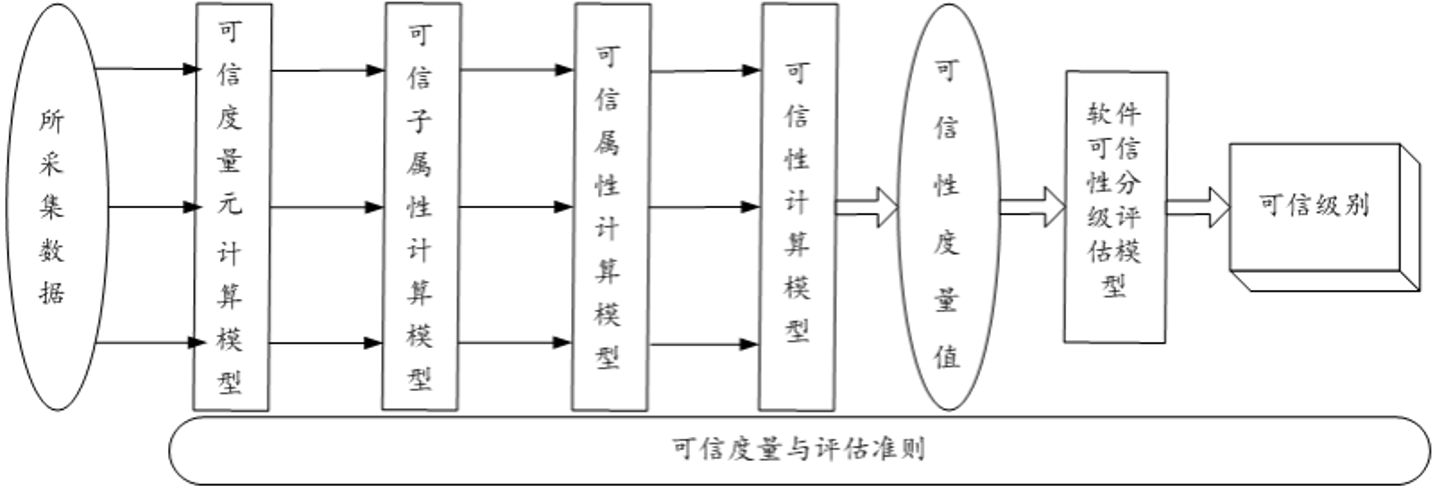
\includegraphics[width=0.9\textwidth]{img/static_2.png}
\end{figure}

在最后一步,通过下述分级模型来判定软件可信等级。

\begin{center}
	\begin{tabular}{|l|l|c|}
		\hline
		\textbf{软件可信度量值要求(黄金分割)} & \textbf{可信属性要求(多数原则)} & \textbf{可信等级} \\ \hline
		$9.5 \leq T$ & 
		\begin{tabular}[c]{@{}l@{}}1. 低于9.5分的关键属性个数不超过 $n - \left\lceil n \cdot \frac{2}{3} \right\rceil$ 个 \\ 2. 没有低于8.5分的可信属性\end{tabular} & V \\ \hline
		\begin{tabular}[c]{@{}l@{}}$8.5 \leq T < 9.5$ 或者 \\ $T > 9.5$ 且不能评为V级别\end{tabular} & 
		\begin{tabular}[c]{@{}l@{}}1. 低于8.5分的关键属性个数不超过 $n - \left\lceil n \cdot \frac{2}{3} \right\rceil$ 个 \\ 2. 没有低于7.0分的可信属性\end{tabular} & IV \\ \hline
		\begin{tabular}[c]{@{}l@{}}$7.0 \leq T < 8.5$ 或者 \\ $T > 8.5$ 且不能评为IV级别及以上者\end{tabular} & 
		\begin{tabular}[c]{@{}l@{}}1. 低于7.0分的关键属性个数不超过 $n - \left\lceil n \cdot \frac{2}{3} \right\rceil$ 个 \\ 2. 没有低于4.5分的可信属性\end{tabular} & III \\ \hline
		\begin{tabular}[c]{@{}l@{}}$4.5 \leq T < 7.0$ 或者 \\ $T > 7.0$ 且不能评为III级别及以上者\end{tabular} & 
		\begin{tabular}[c]{@{}l@{}}1. 低于4.5分的关键属性个数不超过 $n - \left\lceil n \cdot \frac{2}{3} \right\rceil$ 个\end{tabular} & II \\ \hline
		\begin{tabular}[c]{@{}l@{}}$T < 4.5$ 或者 \\ $T > 4.5$ 且不能评为II级别及以上者\end{tabular} & 
		1. 无要求 & I \\ \hline
	\end{tabular}
\end{center}

\subsection{\texttt{Python}代码}

\begin{lstlisting}[language=Python]
	# 插入代码
\end{lstlisting}

\subsection{答案}

\subsubsection{代码运行结果}

\begin{figure}[H]
	\centering
	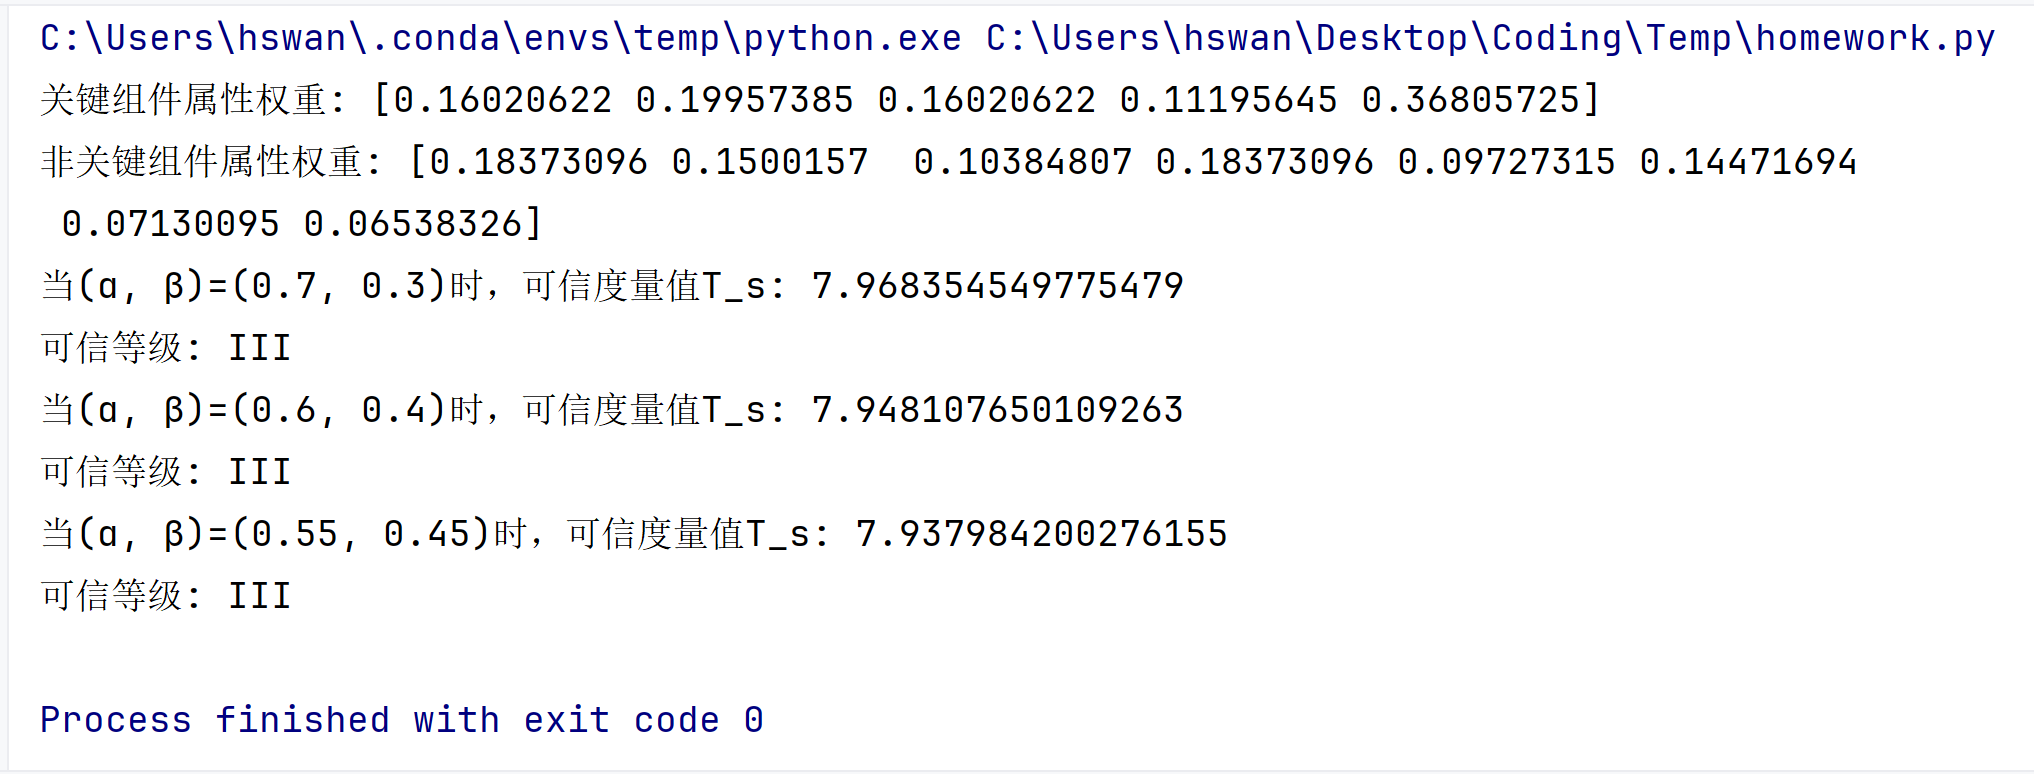
\includegraphics[width=0.9\textwidth]{img/1.png}
	\caption{运行结果}
\end{figure}

\subsubsection{题目答案}

\subsubsection{可视化效果}

\begin{figure}[H]
	\centering
	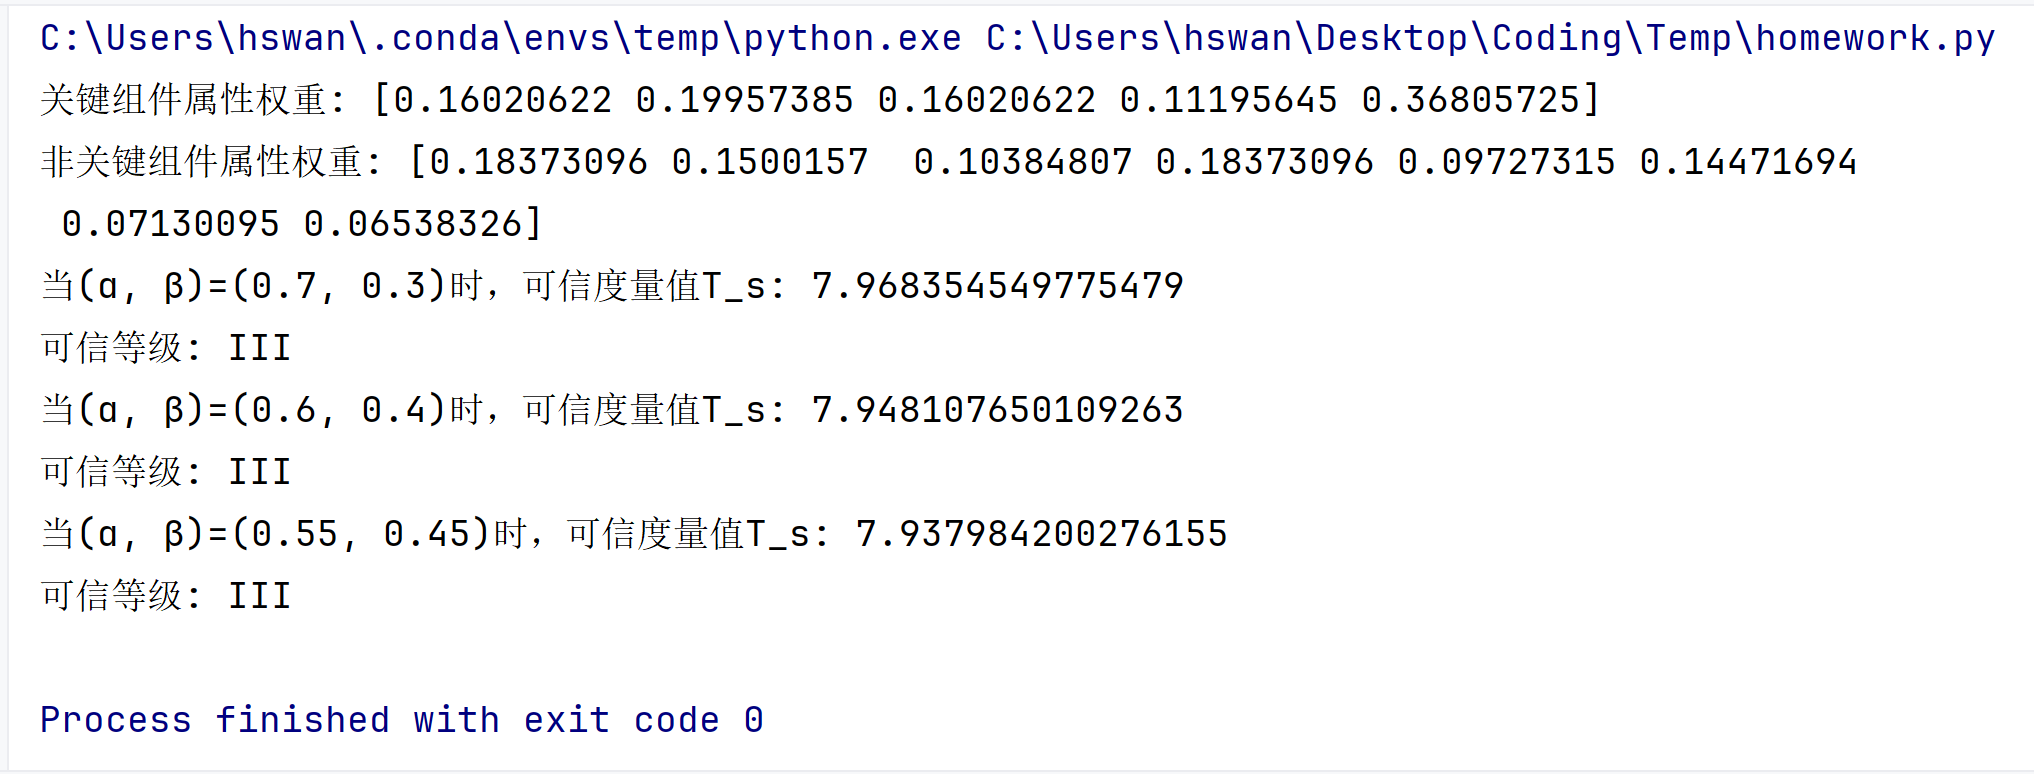
\includegraphics[width=0.9\textwidth]{img/1.png}
	\caption{软件可信属性折线图}
\end{figure}

\begin{figure}[H]
	\centering
	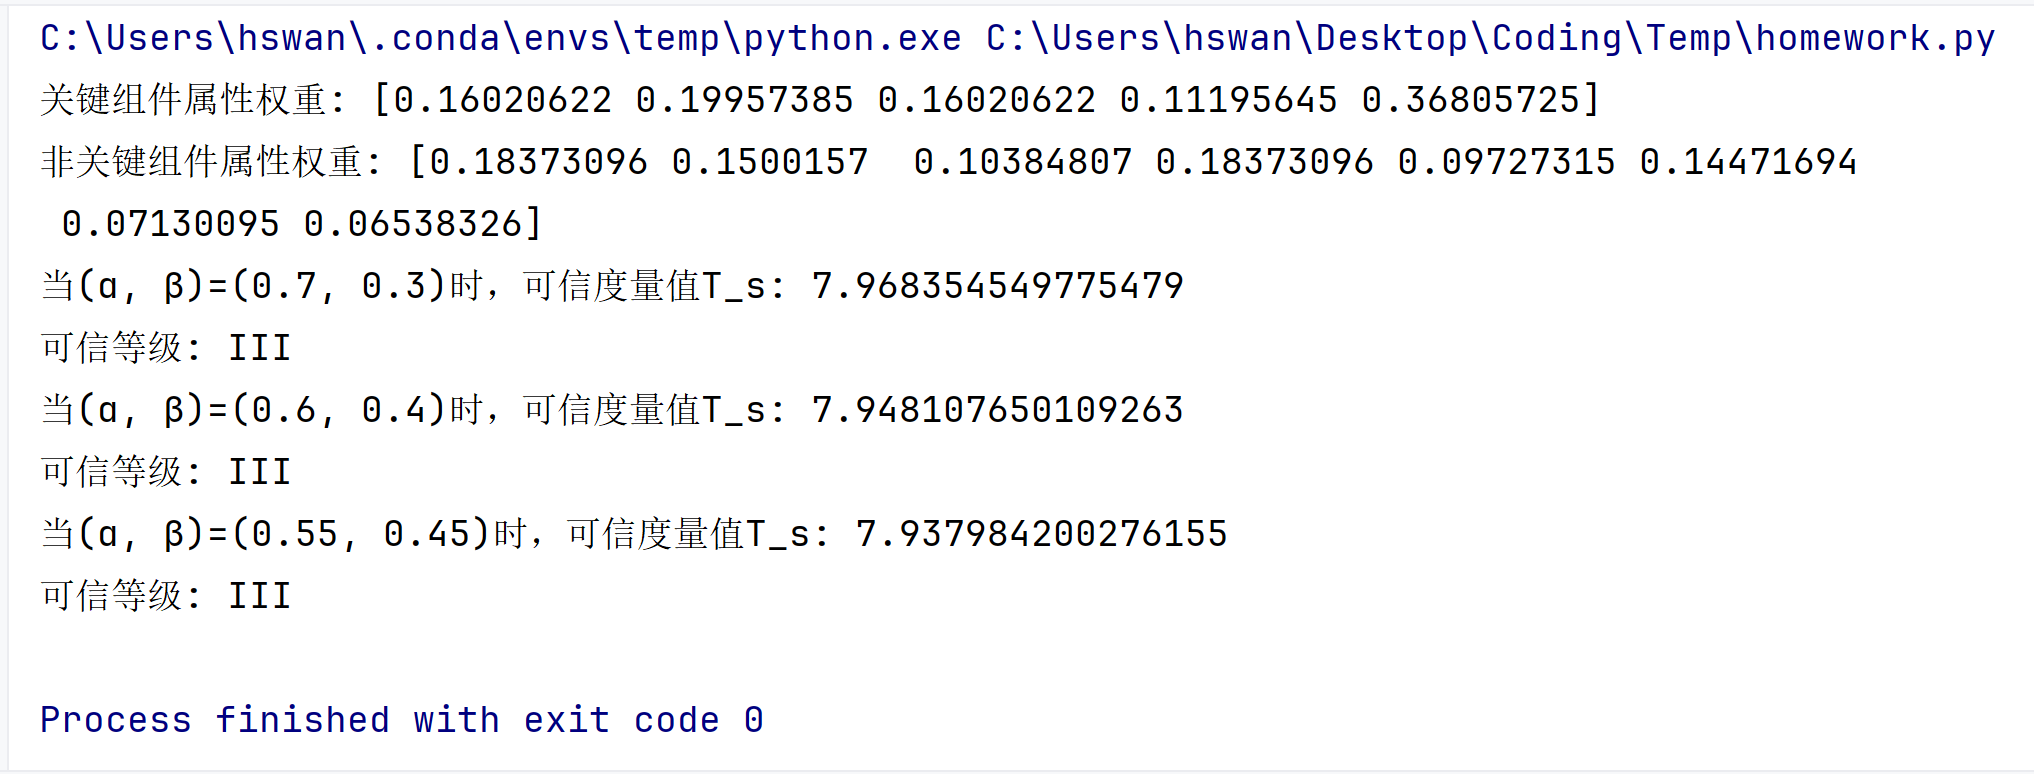
\includegraphics[width=0.9\textwidth]{img/1.png}
	\caption{软件可信等级柱状图}
\end{figure}










\section{hw12-软件老化可信计算框架}

\subsection{题目}

编程或使用课程提供的Python代码,实现下列功能:

\begin{itemize}
	\item \textbf{输入:}类别,以及类别中每个度量元的含例子个数。
	\item \textbf{输出:}在时刻\texttt{t = 0}和\texttt{t = 10}情况下,四个类别的熵和可信度,以及软件可信度.
\end{itemize}

已知的可信属性如下图所示:

\begin{figure}[H]
	\centering
	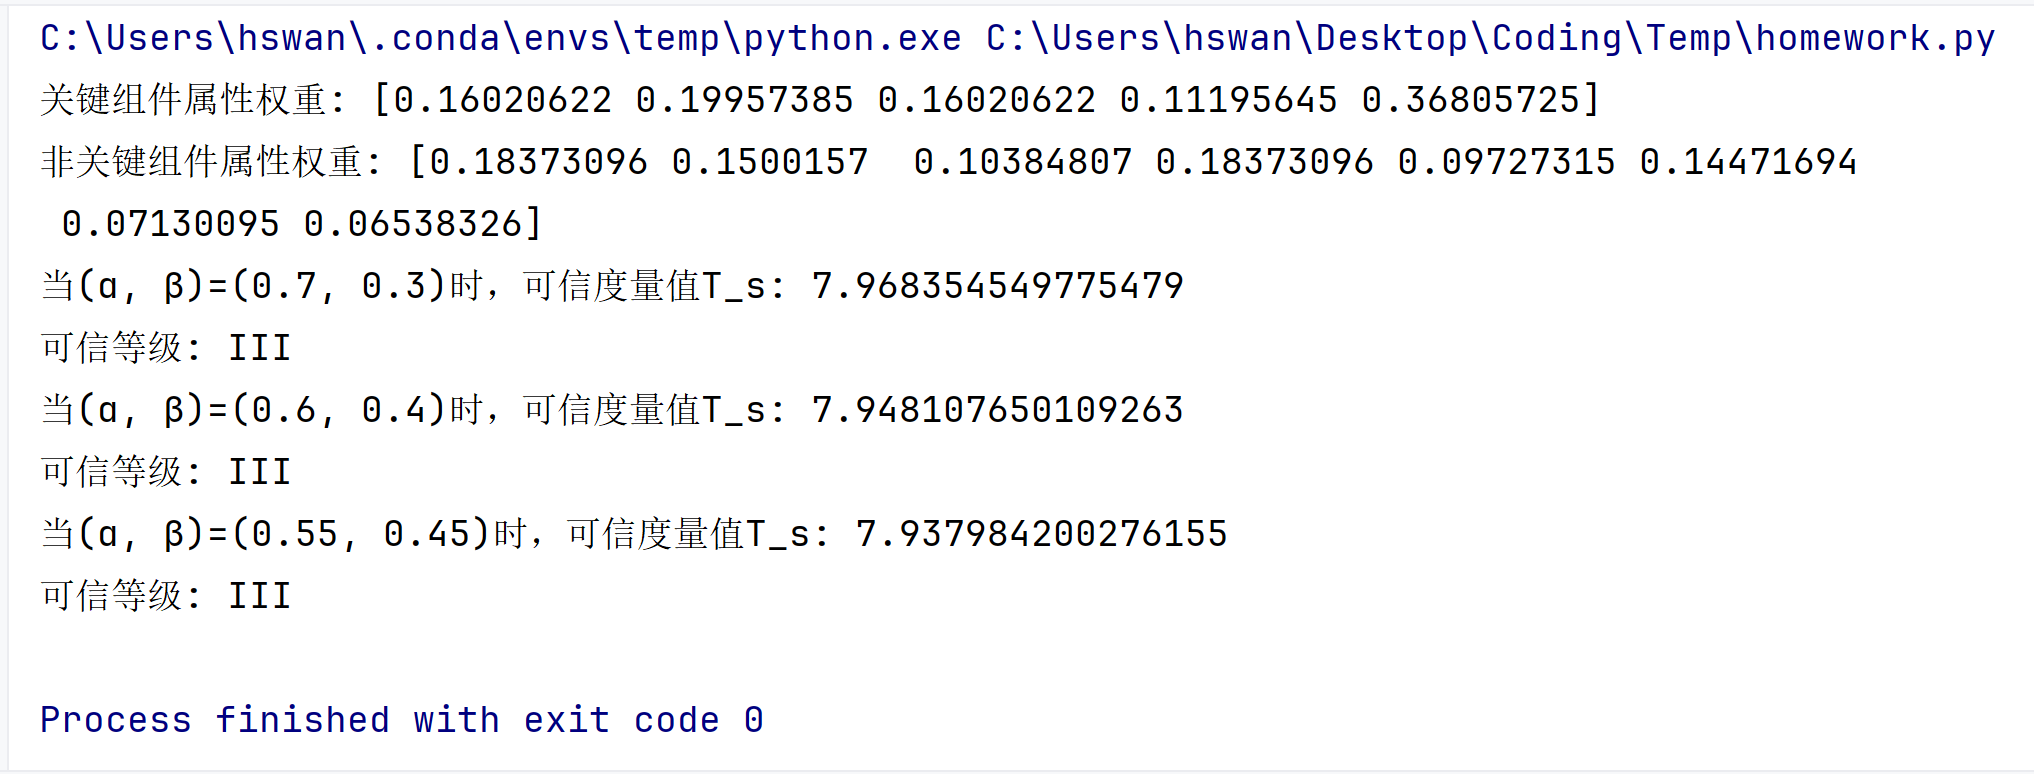
\includegraphics[width=0.9\textwidth]{img/1.png}
	\caption{已知可信属性}
\end{figure}

\subsection{相关知识点}

\begin{figure}[H]
	\centering
	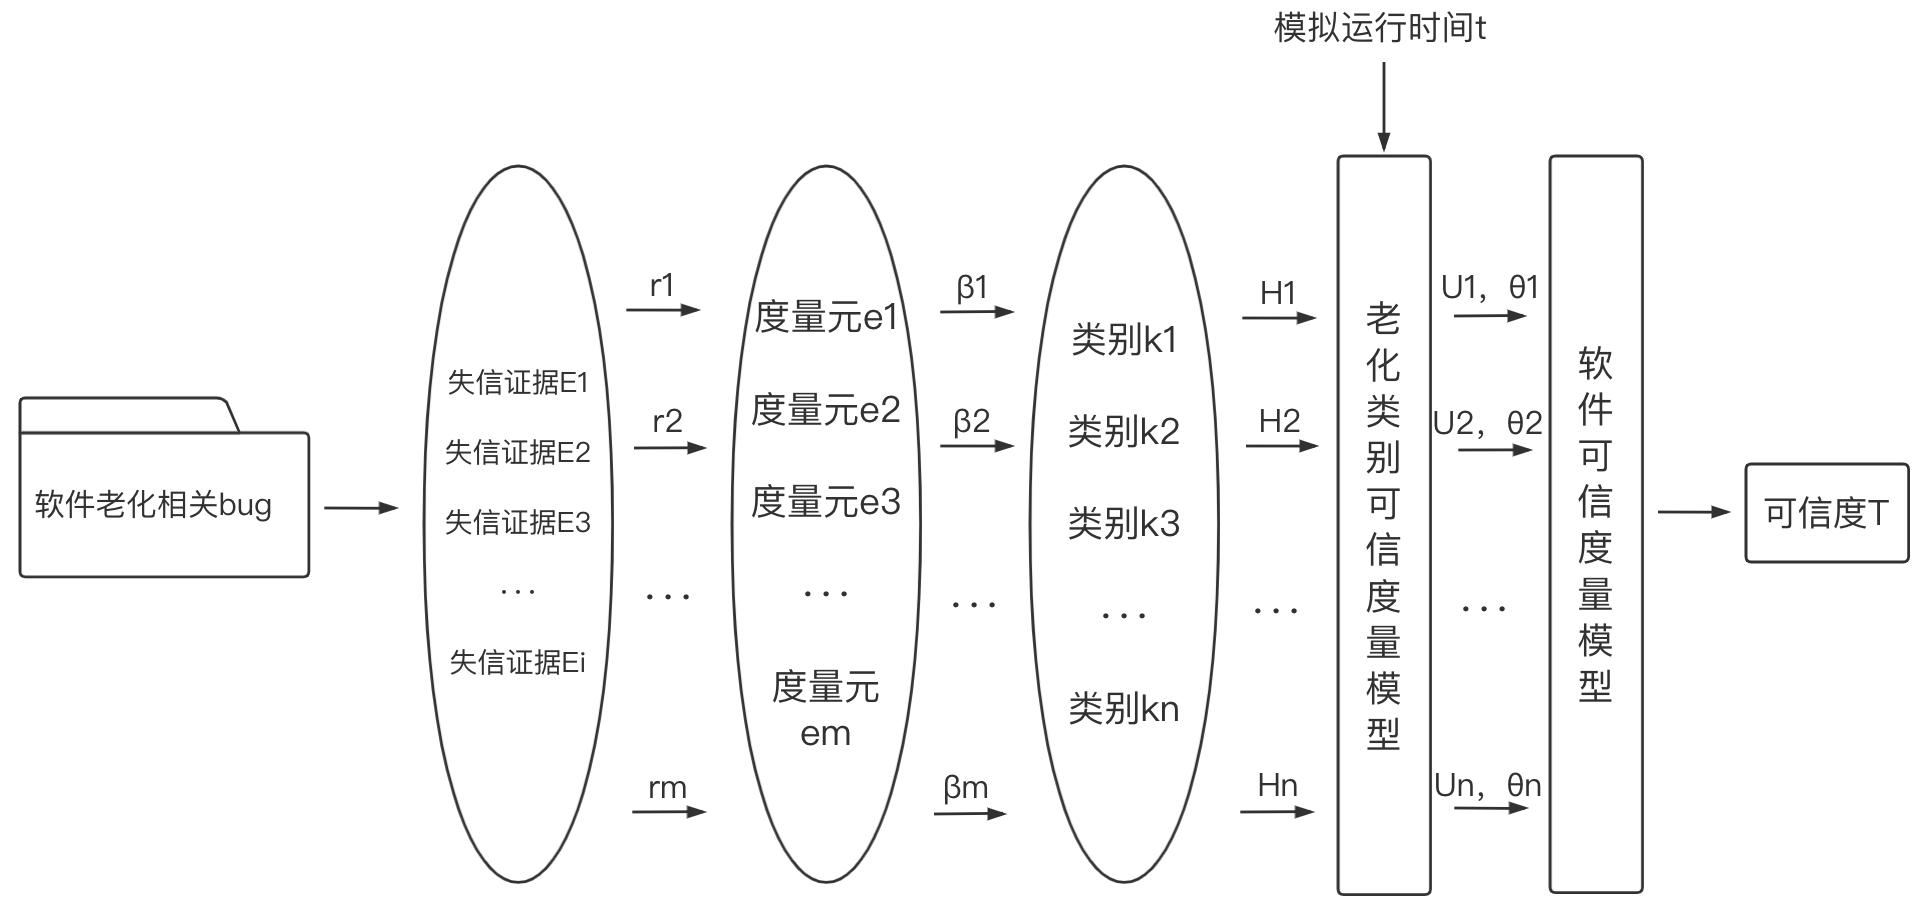
\includegraphics[width=0.9\textwidth]{img/static_3.png}
	\caption{软件老化可信计算框架}
\end{figure}

\subsection{\texttt{Python}代码}

\begin{lstlisting}[language=Python]
	# 插入代码
\end{lstlisting}

\subsection{答案}

\subsubsection{代码运行结果}

\begin{figure}[H]
	\centering
	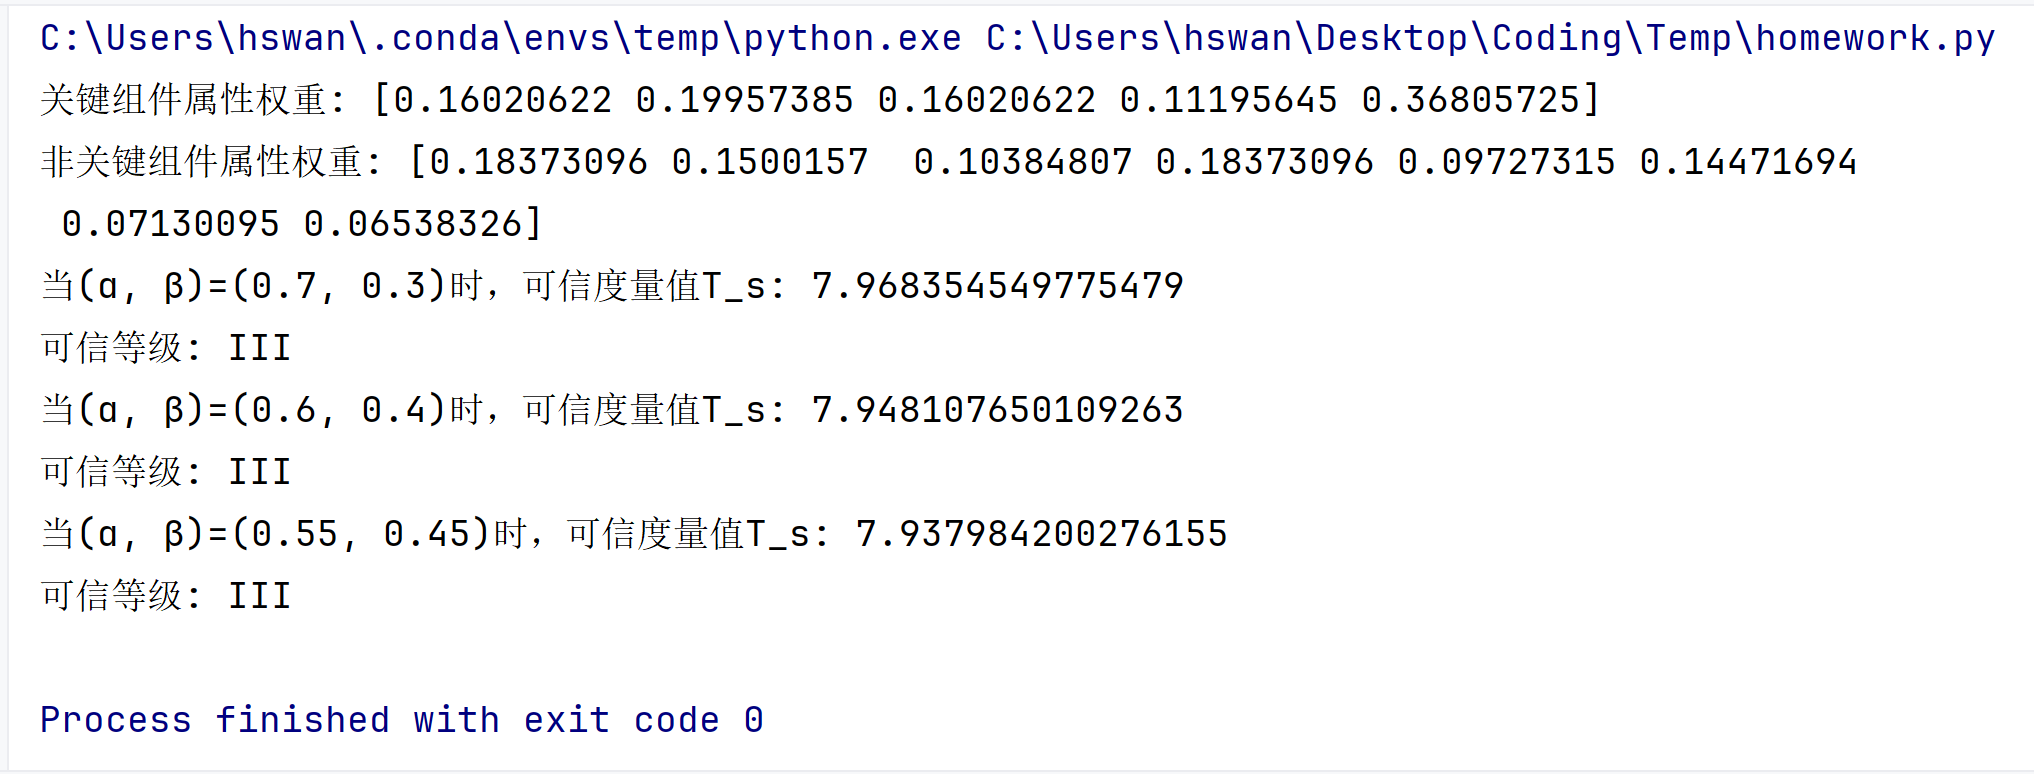
\includegraphics[width=0.9\textwidth]{img/1.png}
	\caption{运行结果}
\end{figure}

\subsubsection{题目答案}












\section{常用格式}

\subsection{图片}

\begin{figure}[H]
	\centering
	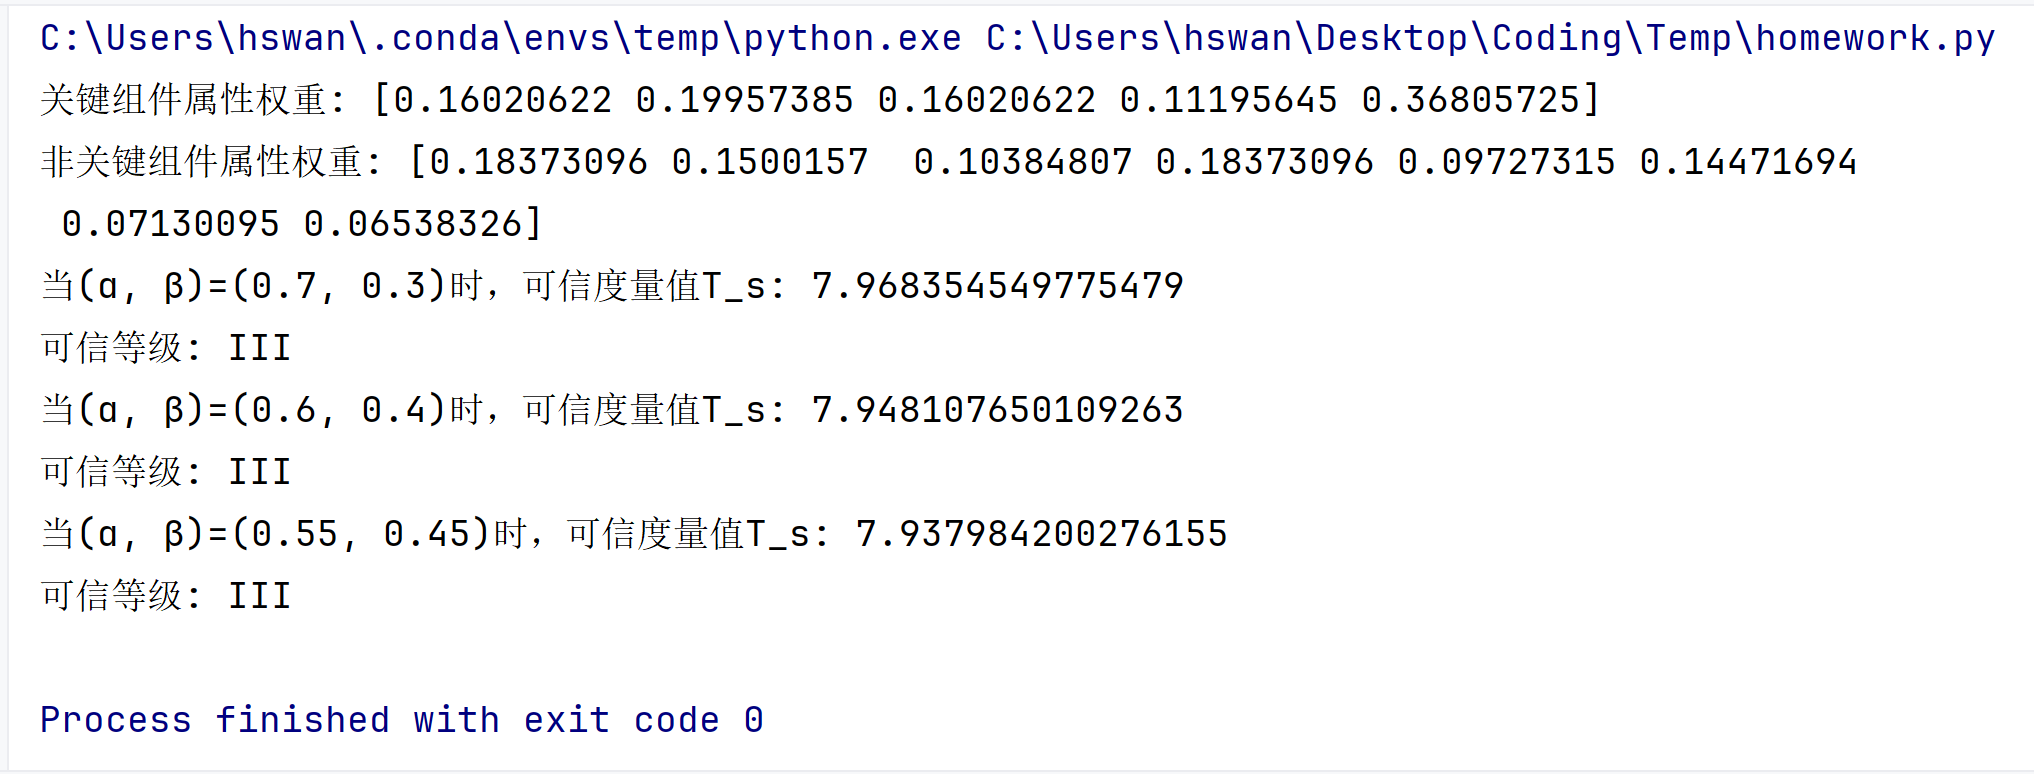
\includegraphics[width=0.9\textwidth]{img/1.png}
	\caption{示例图片}
\end{figure}

\subsection{表格}

\begin{center}
	\begin{tabular}{|c|c|c|c|c|c|c|}
		\hline
		组件名 & CP1 & CP2 & CP3 & CP4 & CP5 & 属性权重 \\
		\hline
		CP1 & 1 & 2 & 1/2 & 2 & 1/4 & \\
		\hline
		CP2 & 1/2 & 1 & 2 & 3 & 1/2 & \\
		\hline
		CP3 & 2 & 1/2 & 1 & 1 & 1/2 & \\
		\hline
		CP4 & 1/2 & 1/3 & 1 & 1 & 1/2 & \\
		\hline
		CP5 & 4 & 2 & 2 & 2 & 1 & \\
		\hline
	\end{tabular}
\end{center}

\subsection{代码块}

\begin{lstlisting}[language=Python]
	import numpy as np
	
	# 计算属性权重的函数,传入正互反判断矩阵
	def calculate_attribute_weights(matrix):
	n = matrix.shape[0]
	
	# 计算几何平均值
	geometric_means = np.power(np.prod(matrix, axis=1), 1 / n)
	
	# 归一化处理
	weights = geometric_means / np.sum(geometric_means)
	return weights
	
	# 1) 计算关键组件和非关键组件的属性权重
	key_weights = calculate_attribute_weights(key_components_matrix)
	non_key_weights = calculate_attribute_weights(non_key_components_matrix)
	
	print("关键组件属性权重:", key_weights)
	print("非关键组件属性权重:", non_key_weights)
\end{lstlisting}

\end{document}